\chapter{Teoria delle perturbazioni}
Fino ad ora si sono discusse teoria di campo libere che danno una descrizione approssimata di molte particelle trovate in Natura. Tuttavia, stati di particella libera sono autostati dell'hamiltoniana e non si è parlato né di interazione né di scattering. In modo da ottenere una descrizione più accurata del mondo reale si devono necessariamente includere nuovi termini non lineari nell'hamitoniana o nella lagrangiana che accoppiano differenti modi di Fourier, e le particelle che li occupano, l'uno con l'altro. Per conservare la causalità, si insiste sulla condizione che questi nuovi termini devono includere solamente prodotti dei campi e dello loro derivate calcolate nello stesso punto dello spaziotempo. Quindi, l'hamiltoniana che include i termini descriventi l'interazione ha la forma
\begin{equation}
    \hatH' = \int d^3x\,\SH'[\hatphi(x),\p_\mu\hatphi(x)] = -\int d^3x\,\dL'[\hatphi(x),\p_\mu\hatphi(x)].
\end{equation}
Si intende ora studiare la Teoria delle perturbazioni per campi interagenti con l'obiettivo di arrivare ad un formalismo che permetta di visualizzare le serie perturbative come processi dello spaziotempo. Pur non avendo necessità di riformulare la Meccanica quantistica, si intende derivare una ``nuova'' Teoria delle perturbazioni dipendenti dal tempo conveniente per una teoria di campo. Il risultato a cui si intende arrivare è il calcolo delle sezioni d'urto dei processi di scattering e le frequenze di decadimento, ma per ora ci si concentra sul calcolare la più semplice, anche se più astratta, funzioni di Green a due punti 
\begin{equation}
    \mybrakett{\Omega}{T[\hatphi(x)\hatphi(y)]}{\Omega}.
\end{equation}
Per una teoria libera si era determinato che il propagatore di un campo scalare, sia carico che neutro, ha la forma trovata nell'equazione \eqref{eq: propagatore libero campo scalare carico}, quindi si vuole capire come tale espressione cambi in una teoria interagente e quale sia la relazione che la lega al propagatore libero. Per farlo, prima di tutto si scrive l'hamiltoniana del sistema come la somma tra quella libera e quella di interazione
\begin{equation}
    \hatH = \hatH_0 + \hatH',\quad \hatH' \ll 1,
\end{equation}
dove la condizione imposta sull'hamiltoniana di interazione è fondamentale per sviluppare una teoria perturbativa, infatti in questo modo si sta considerando un'interazione ``piccola'' e presente per un tempo molto limitato, in modo da poter sviluppare in serie i termini di interazione. Tale condizione è anche legata al fatto che in generale in Teoria dei campi le interazioni sono descritte come lo scambio di particelle ``virtuali'', ossia particelle che non rispettano l'equazione di mass-shell della Relatività speciale violando quindi la conservazione dell'energia; potrebbe sembrare impossibile, ma in realtà questa violazione è giustificata dal fatto che queste particelle vivono per un tempo tale da soddisfare la relazione di indeterminazione tra energia e tempo $\Delta E \Delta t  \simeq \hbar$. Ora per descrivere l'evoluzione temporale di stati ed operatori si fa uso di una particolare rappresentazione detta ``di interazione'' in cui gli stati $\ket{\psi_I}$ evolvono unicamente con l'hamiltoniana di interazione $\hatH'$, mentre gli operatori $\hatO$ evolvono unicamente con l'hamiltoniana libera $\hatH_0$; in questo modo gli operatori evolvono secondo
\begin{equation}
    \hatO_I(t) = e^{i\hatH_0t}\hatO e^{-i\hatH_0t}
\end{equation}
ottenendo così un'equazione del moto alla Heisenberg per l'hamiltoniana libera
\begin{equation}
    i\frac{d\hatO_I}{dt} = \comm{\hatO_I(t)}{\hatH_0},
\end{equation}
invece gli stati soddisfano l'equazione di Schr\"odinger per l'hamiltoniana di interazione
\begin{equation}
    i\frac{\p}{\p t}\ket{\psi_I(t)} = \hatH'_I\ket{\psi_I(t)},\quad \hatH_I' = e^{i\hatH_0t}\hatH' e^{-i\hatH_0t}.
\end{equation}
Stabilita l'evoluzione temporale degli operatori, si considera un generico elemento di matrice nella rappresentazione di Schr\"odinger e lo si confronta con uno in quella di interazione in modo da verificare che queste rappresentazioni siano equivalenti
\begin{equation}
    \begin{split}
        \mybrakett{\phi(t)}{\hatO}{\psi(t)}&=\mybrakett{\phi(0)}{\hatU^\dagger(t,0)\hatO\hatU(t,0)}{\psi(0)} \\
        &=\mybrakett{\phi(0)}{e^{i\hatH t}\hatO e^{-i\hatH t}}{\psi(0)} \\
        &=\mybrakett{\phi(0)}{e^{i\hatH' t}e^{i\hatH_0 t}\hatO e^{-i\hatH_0 t}e^{-i\hatH' t}}{\psi(0)} \\
        &=\mybrakett{\phi_I(t)}{e^{i\hatH_0 t}\hatO e^{-i\hatH_0 t}}{\psi_I(t)},
    \end{split}
\end{equation}
quindi i valori medi di ogni elemento di matrice sono gli stessi in qualsiasi rappresentazione
\begin{equation}
    \underbrace{\mybrakett{\phi(t)}{\hatO}{\psi(t)}}_{\substack{Schr\ddot{o}dinger\\picture}}\equiv\underbrace{\mybrakett{\phi_I(t)}{e^{i\hatH_0t}\hatO e^{-i\hatH_0t}}{\psi_I(t)}}_{\substack{interaction\\picture}}.
\end{equation}
\begin{obs}
    Al tempo $t=0$ tutte le rappresentazioni, Schr\"odinger, Heisenberg ed interazione, coincidono.
\end{obs}
La rappresentazione di interazione è utile in quanto l'hamiltoniana di interazione $\hatH'$ è nulla all'inizio e alla fine del processo. Infatti, si supponga che $\hatH'$ si ``accenda'' e si ``spenga'' in modo continuo senza interruzioni. Quando $\hatH_I=0$ l'unica rappresentazione presente è quella di Heisenberg per l'hamiltoniana libera $\hatH_0$. Quindi, gli autostati di $\hatH_0$ sono $\ket{\psi_I(\pm\infty)}$, i quali possono essere costruiti a partire dallo stato di vuoto $\sv$ applicando gli operatori di creazione o distruzione. Inoltre, l'hamiltoniana di interazione è diversa da zero solo durante il breve intervallo di tempo in cui avviene l'interazione tra particelle, per poi tornare nuovamente a zero, quindi $\hatH'=0$ per $t\to\pm\infty$. In questo modo, è possibile dare una rappresentazione funzionale dell'hamiltoniana di interazione
\begin{equation}
    \hatH_I(t)=\lambda(t)\hatH'.
\end{equation}
\begin{figure}[h]
    \centering
    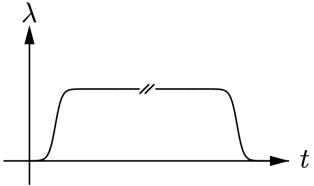
\includegraphics[width=0.5\linewidth]{Immagini/rappr. ham. int.png}
    \caption{rappresentazione funzionale dell'hamiltoniana di interazione.}
    \label{fig: rappr. ham. int.}
\end{figure}

Ricapitolando, gli stati evolvono nel tempo solo durante il periodo in cui avviene l'interazione secondo $\hatH'$, o meglio $\hatH_I$, nel quale $\hatH_I\neq0$; al di fuori di tale intervallo gli stati sono stazionari, mentre gli operatori evolvono nel tempo secondo $\hatH_0$.

Quindi, essendo i campi degli operatori la loro evoluzione temporale in rappresentazione di Heisenberg è data da
\begin{equation}
    \hatphi(\vx,t) = e^{i\hatH(t - t_0)}\hatphi(\vx,t_0)e^{-i\hatH(t - t_0)},
\end{equation}
scegliendo un istante di tempo fissato $t_0$ è possibile esprimere il campo tramite la sua espressione esplicita \eqref{eq: campo scalare quantizzato} in termini di operatori di creazione e distruzione, in particolare per $\lambda(t) = 0$, l'hamiltoniana $\hatH$ si riduce ad $\hatH_0$ e l'evoluzione temporale del campo in rappresentazione di interazione, come ci si aspetta, è
\begin{equation}
    \hatphi_I(\vx,t) \equiv e^{i\hatH_0(t - t_0)}\hatphi(\vx,t_0)e^{-i\hatH_0(t - t_0)};
\end{equation}
quando $\lambda(t) \ll 1$ questa espressione continua a restituire la parte più importante della dipendenza temporale del campo $\hatphi(x)$ e quindi è possibile usarla in una teoria perturbativa. Adesso si deve esprimere il campo $\hatphi(x)$ in termini di $\hatphi_I(x)$, quindi
\begin{equation}
    \begin{split}
        \hatphi(x) &= e^{i\hatH(t - t_0)}e^{-i\hatH_0(t - t_0)}\hatphi_I(x)e^{i\hatH_0(t - t_0)}e^{i\hatH(t - t_0)} \\
        &= \hatU^\dg_I(t,t_0)\hatphi_I(t)\hatU_I(t,t_0),
    \end{split}
\end{equation}
dove si è definito l'operazione di evoluzione temporale in rappresentazione di interazione $\hatU_I(t,t_0)$ come
\begin{equation}
    \hatU_I(t,t_0) := e^{i\hatH_0(t - t_0)}e^{-i\hatH(t - t_0)}.
\end{equation}
Anche $\hatU_I(t,t_0)$ deve essere espresso in termini di $\hatphi_I(x)$ di cui si conosce la forma esplicita. Per farlo, si osserva che $\hatU(t,t_0)$ è soluzione, con condizione iniziale $\hatU_I(t_0,t_0) = 1$, dall'equazione di Schr\"odinger
\begin{equation}
    \begin{split}
        i\frac{\p}{\p t}\hatU_I(t,t_0) &= e^{i\hatH_0(t - t_0)}(\hatH - \hatH_0)e^{-i\hatH(t-t_0)} \\
        &= e^{i\hatH_0(t - t_0)}\hatH'e^{-i\hatH(t - t_0)} \\
        &= e^{i\hatH_0(t - t_0)}\hatH'e^{-i\hatH_0(t - t_0)}e^{i\hatH_0(t - t_0)}e^{-i\hatH(t - t_0)} \\
        &= \hatH_I'(t)\hatU_I(t,t_0).
    \end{split}
\end{equation}
La soluzione di tale equazione non è semplicemente dato dall'esponenziale $\hatU(t,t_0) = \exp{(-i\int_{t_0}^t\hatH_I'(t')\,dt')}$ dato che l'hamiltoniana di interazione non commuta a tempi diversi, infatti in verità si ha
\begin{equation}
    \hatU(t,t_0) = 1 + (-i)\int_{t_0}^tdt_1\,\hatH_I'(t_1) + (-i)^2 \int_{t_0}^t\int_{t_0}^{t_1}dt_1\,dt_2\,\hatH_I'(t_1)\hatH_I'(t_2) + \cdots,
\end{equation}
che può essere riscritta tramite l'operatore di ordinamento temporale \eqref{eq: ordinamento temporale} nella forma più compatta
\begin{equation}
    \hatU(t,t_0) = T\bigg[\exp{\bigg(-i\int_{t_0}^tdt'\,\hatH'_I(t')\bigg)}\bigg],
\end{equation}
dove l'operatore $T$ è definito come la serie di Taylor avente ogni termine ordinato temporalmente. 

Si vuole adesso trovare una relazione tra lo stato fondamentale interagente $\kO$ e lo stato di vuoto $\sv$. Siccome l'energia minima di una teoria libera è posta a zero, allora $\hatH_0\sv = 0$. Considerando il termine di interazione $\hatH = \hatH_0 + \hatH'$, si definiscono ${\ket{n}}$ come gli autostati di $\hatH$ dotati di una relazione di completezza 
\begin{equation}
    \nsum_n\ket{n}\bra{n} = \MI,
\end{equation}
tra questi autostati esiste uno stato $\kO$ che appunto rappresenta lo stato fondamentale della teoria interagente tale per cui
\begin{equation}
    \hatH\kO = E_0\kO.
\end{equation}
Lo stato $\kO$ può essere espresso come una sovrapposizione lineare, potenzialmente infinita, di autostati dell'impulso di $\hatH_0$. Tra tutti questi ulteriori autostati di $\hatH_0$ è presente anche lo stato di vuoto $\sv$, per cui $\kO$ è parzialmente sovrapposto a $\sv$ e quindi $\mybraket{\Omega}{0} \neq 0$. Per isolare $\kO$ si parte pertanto dall'evolvere lo stato $\sv$ tramite $\hatH$ per un tempo $T$ ottenendo
\begin{equation}
    \begin{split}
        e^{-i\hatH T}\sv &= e^{-i\hatH T}\nsum_n\ket{n}\mybraket{n}{0} \\
        &= \nsum_n e^{-iE_nT}\ket{n}\mybraket{n}{0} \\
        &= e^{-iE_0T}\kO\mybraket{\Omega}{0} + \nsum_{n\neq0}e^{-iE_nT}\ket{\mybraket{n}{0}}.
    \end{split}
\end{equation}
Dato che per ogni $n\neq0$, $E_n > E_0$, allora ci si può sbarazzare dei termini con $n\neq0$ considerando il limite complesso per $T\to\infty(1 - i\epsilon)$ e, dato che il termine con $e^{iE_0t}$ è quello che decresce più lentamente, si ha
\begin{equation}
    \kO = \lim_{T\to\infty(1 - i\epsilon)}(e^{-iE_0T}\mybraket{\Omega}{0})^{-1}e^{-i\hatH T}\sv.
\end{equation}
Dato che $T\to\infty(1 - i\epsilon) \equiv \infty^\C$, allora si può considerare una traslazione temporale $T\to T + t_0$, con $t_0\in\R$, in questo modo
\begin{equation}
    \begin{split}
        \kO &= \lim_{T\to\infty^\C}(e^{-iE_0(T + t_0)}\mybraket{\Omega}{0})^{-1}e^{-i\hatH (T + t_0)}\sv \\
        &= \lim_{T\to\infty^\C}(e^{-iE_0(t_0 - (-T))}\mybraket{\Omega}{0})^{-1}e^{-i\hatH (t_0 - (-T))}\sv \\
        &= \lim_{T\to\infty^\C}(e^{-iE_0(t_0 - (-T))}\mybraket{\Omega}{0})^{-1}e^{-i\hatH (t_0 - (-T))}e^{i\hatH_0(t_0 - (-T))}\sv \\
        &= \lim_{T\to\infty^\C}(e^{-iE_0(t_0 - (-T))}\mybraket{\Omega}{0})^{-1}\hatU(t_0,-T)\sv,
    \end{split}
\end{equation}
dove la definizione $\hatU(t_0,-T) := e^{-i\hatH (t_0 - (-T))}e^{i\hatH_0(t_0 - (-T))}$ vale in quanto per $T\to\infty^\C$ si ha $\hatH\simeq\hatH_0$ e $\hatH'\to0$. Analogamente, si può esprimere 
\begin{equation}
    \bO = \lim_{T\to\infty^\C}\bra{0}\hatU(T,t_0)(e^{-iE_0(T - t_0)}\mybraket{0}{\Omega})^{-1}.
\end{equation}
Ora che sono note le espressioni degli stati $\kO$ e $\bO$ in funzione di $\sv$ e $\bra{0}$ insieme a quelle dei campi $\hatphi(x)$ in funzione di $\hatphi_I(x)$ è possibile determinare la forma del propagatore interagente, quindi
\begin{equation}
    \begin{split}
        \mybrakett{\Omega}{T[\hatphi(x)\hatphi(y)]}{\Omega} &= \lim_{T\to\infty^\C}(|\mybraket{0}{\Omega}|^2e^{-2iE_0T})^{-1} \times \\
        &\times\mybrakett{0}{\hatU(T,x^0)\hatphi_I(x)\hatU(x^0,y^0)\hatphi_I(y)\hatU(y^0,-T)}{0},
    \end{split}
\end{equation}
dove per il momento si è supposto che $x^0 > y^0 > t_0$. Adesso dividendo per la normalizzazione dello stato fondamentale 
\begin{equation}
    \mybraket{\Omega}{\Omega} = (|\mybraket{0}{\Omega}|^2e^{-2iE_0T})^{-1}\mybrakett{0}{\hatU(T,t_0)\hatU(t_0,-T)}{0} = 1,
\end{equation}
si ottiene 
\begin{equation}
    \mybrakett{\Omega}{T[\hatphi(x)\hatphi(y)]}{\Omega} = \lim_{T\to\infty^\C}\frac{\mybrakett{0}{\hatU(T,x^0)\hatphi_I(x)\hatU(x^0,y^0)\hatphi_I(y)\hatU(y^0,-T)}{0}}{\mybrakett{0}{\hatU(T,t_0)\hatU(t_0,-T)}{0}}.
\end{equation}
Quest'ultima però non è ancora l'espressione completa dato che non si sta rispettando necessariamente la causalità, come al solito si deve introdurre l'operatore di ordinamento temporale per rispettarla ottenendo finalmente l'espressione del propagatore di una teoria interagente in funzione dello stato di vuoto di una teoria libera
\begin{equation}
\label{eq: teorema di Gell-Mann - Low}
    \mybrakett{\Omega}{T[\hatphi(x)\hatphi(y)]}{\Omega} = \lim_{T\to\infty^\C}\frac{\mybrakett{0}{T[\hatphi_I(x)\hatphi_I(y)\exp{(-i\int_{-T}^Tdt\,\hatH_I(t))}]}{0}}{\mybrakett{0}{T[\exp{(-i\int_{-T}^Tdt\,\hatH_I(t)}]}{0}}.
\end{equation}
L'incredibile e fondamentale risultato mostrato nella \eqref{eq: teorema di Gell-Mann - Low} è codificato formalmente nel teorema di Gell-Mann - Low nella Teoria dei campi. Il risultato trovato è chiaramente estendibile ad un numero arbitrario di campi; per ogni fattore ulteriore $\hatphi$ nel membro sinistro si aggiunge un fattore $\hatphi_I$ in quello di destra. Oltre ad essere un'espressione esatta, è anche adatta per svolgere calcoli perturbativi: serve solamente troncare la serie di Taylor degli esponenziali all'ordine a cui si è interessati.

\section{Teorema di Wick}
Le quantità che spesso si devono calcolare per determinare le ampiezze di scattering $\amp$ di una determinata teoria sono valori di aspettazione di un prodotto T-ordinato di un certo numero di campi, ossia oggetti del tipo
\begin{equation}
    \mybrakett{0}{T[\hatphi_I(x_1)\cdots\hatphi_I(x_n)]}{0}.
\end{equation}
Questo tipo di calcoli è in generale molto complesso, ma il teorema di Wick semplifica notevolmente la procedura. Questo mette in relazione il valore di aspettazione sullo stato di vuoto del prodotto T-ordinato con quello del prodotto ``normal ordered'', il quale è sempre nullo dato che l'ordinamento normale pone gli operatori di distruzione a destra e quelli di creazione a sinistra, rendendo il valore di aspettazione sul vuoto nullo.

Quindi, si parte considerando, ad esempio, l'espressione dell'operatore di campo $\hatphi$ in \eqref{eq: campo scalare quantizzato} e osservando che è composto da due parti, una di distruzione e una di creazione, pertanto $\hatphi$ può essere scritto come la somma di tali parti $\hatphi=\hatphi^++\hatphi^-$, in modo da avere $\hatphi^-\sv=\bra{0}\hatphi^+=0$ e quindi definite come
\begin{align}
\label{componenti campo + e -}
    \hatphi^+(x) &= \int\frac{d^3k}{(2\pi)^{3/2}}\frac{1}{(2\omega_k)^{1/2}}\hata_k^\dg e^{ik_\mu x^\mu}, \\
    \hatphi^-(x) &= \int\frac{d^3k}{(2\pi)^{3/2}}\frac{1}{(2\omega_k)^{1/2}}\hata_ke^{-ik_\mu x^\mu}.
\end{align}

Si consideri ora il caso più semplice di due operatori di campo $\hatphi_A$ e $\hatphi_B$. Il loro prodotto è dato da 
\begin{equation}
    \hatphi_A\hatphi_B=(\hatphi_A^++\hatphi_A^-)(\hatphi_B^++\hatphi_B^-)=\hatphi_A^+\hatphi_B^++\hatphi_A^-\hatphi_B^-+\hatphi_A^+\hatphi_B^-+\hatphi_A^-\hatphi_B^+.
\end{equation}
Nel caso di prodotto normalmente ordinato si ha
\begin{equation}
    N[\hatphi_A\hatphi_B]=\hatphi_A^+\hatphi_B^++\hatphi_A^-\hatphi_B^-+\hatphi_A^+\hatphi_B^-+\hatphi_B^+\hatphi_A^-.
\end{equation}
Il passo fondamentale è notare che la differenza tra questi due prodotti è
\begin{equation}
    \hatphi_A\hatphi_B-N[\hatphi_A\hatphi_B=\comm{\hatphi_A^-}{\hatphi_B^+}.
\end{equation}
Ricordando che $\hatphi_A$ e $\hatphi_B$ sono operatori di campo, il loro prodotto deve essere T-ordinato, quindi
\begin{equation}
    T[\hatphi_A(x^\mu)\hatphi_B(y^\mu)]=
    \begin{cases}
        \hatphi_A(x^\mu)\hatphi_B(y^\mu),\quad x^0>y^0 \\
        \hatphi_B(y^\mu)\hatphi_A(x^\mu),\quad y^0>x^0
    \end{cases}.
\end{equation}
Facendo ora la differenza tra il prodotto T-ordinato con quello normalmente ordinato si ottiene
\begin{equation}
    T[\hatphi_A(x^\mu)\hatphi_B(y^\mu)]-N(\hatphi_A\hatphi_B)=
    \begin{cases}
        \comm{\hatphi_A^-(x^\mu)}{\hatphi_B^+(y^\mu)},\quad x^0>y^0 \\
        \comm{\hatphi_B^-(y^\mu)}{\hatphi_A^+(x^\mu)},\quad y^0>x^0
    \end{cases}.
\end{equation}
Dato che il valore di aspettazione sullo stato di vuoto di un prodotto normalmente ordinato è sempre nullo, si può scrivere che il valore di aspettazione del prodotto T-ordinato come
\begin{equation}
    \mybrakett{0}{T[\hatphi_A(x^\mu)\hatphi_B(y^\mu)]}{0}=
    \begin{cases}
        \mybrakett{0}{\comm{\hatphi_A^-(x^\mu)}{\hatphi_B^+(y^\mu)}}{0},\quad x^0>y^0 \\
        \mybrakett{0}{\comm{\hatphi_B^-(y^\mu)}{\hatphi_A^+(x^\mu)}}{0},\quad y^0>x^0
    \end{cases}.
\end{equation}
In generale, si definisce la differenza tra il prodotto T-ordinato ed N-ordinato come una contrazione
\begin{equation}
\label{eq: definizione contrazione}
    \overbracket{\hatphi_A\hatphi_B}=T[\hatphi_A\hatphi_B]-N[\hatphi_A\hatphi_B].
\end{equation}
Dato che il prodotto normale non ha alcun effetto sul valore di aspettazione sullo stato di vuoto, si può scrivere che
\begin{equation}
    \label{eq: relazione tra contraz. e VEV}
    \overbracket{\hatphi_A\hatphi_B}=\overbracket{\hatphi_A\hatphi_B}\mybraket{0}{0}=\mybrakett{0}{\overbracket{\hatphi_A\hatphi_B}}{0}=\mybrakett{0}{T[\hatphi_A\hatphi_B]}{0}.
\end{equation}
Questo risultato può essere generalizzato con il seguente teorema.
\begin{teo}[teorema di Wick]
    Il prodotto T-ordinato di $n$ operatori $\hatphi_I(x_i) \equiv \hatphi_i$ è uguale al prodotto normale degli $n$ operatori più il prodotto normale della somma di tutti i possibili modi di contrarre gli operatori tra loro, ovvero
    \begin{equation}
        T[\hatphi_1\dots\hatphi_n] = N[\hatphi_1\dots\hatphi_n] + N[\mathrm{tutte\,le\,possibili\,contrazioni}].
    \end{equation}
\end{teo}
\begin{proof}
    Per prima cosa si nota che il prodotto T-ordinato di $n$ operatori di campo $\hatphi_I$ è invariante sotto lo scambio dei campi per definizione. Dato che i prodotti N-ordinati e le contrazioni sono invarianti sotto lo scambio dei campi è possibile, senza perdere di generalità, scegliere $x_{n + 1}^0 < x_i^0$ con $i\in\{1,\dots,n\}$. Assumendo che il teorema di Wick sia vero per $n$ operatori di campo si ha
    \begin{equation}
        \begin{split}
            T[\hatphi_1\dots\hatphi_{n+1}] &= T[\hatphi_1\dots\hatphi_n]\hatphi_{n+1} \\
            &= N[\hatphi_1\dots\hatphi_n]\hatphi_{n+1} + \sum_{\mathrm{perm}}\mybrakett{0}{T[\hatphi_1\hatphi_2]}{0}N[\hatphi_3\cdots\hatphi_n]\hatphi_{n+1}.
        \end{split}
    \end{equation}
    Finora $\hatphi_{n+1}$ è rimasto fuori dai prodotti N-ordinati; ora si deve operare in modo da portalo all'interno di tali prodotti. Per farlo si usano le definizioni \eqref{componenti campo + e -} e si nota che un prodotto N-ordinato ha sempre i campi $\hatphi^-$ a destra e i campi $\hatphi^+$ a sinsitra, per cui
    \begin{equation}
        N[\hatphi_1\cdots\hatphi_n] = \sum_{A,B}\prod_{i\in A}\prod_{j\in B}\hatphi^+_i\hatphi_j^-,
    \end{equation}
    dove $A$ e $B$ rappresentano le partizioni dell'insieme di $1,2,\dots,n$ elementi. Con questa notazione si può scrivere
    \begin{equation}
    \label{eq: prodotto N-ordinato Wick's proof}
        N[\hatphi_1\cdots\hatphi_m]\hatphi_{n+1} = \bigg[\sum_{A,B}\prod_{i\in A}\prod_{j\in B}\hatphi^+_i\hatphi_j^-\bigg](\hatphi^+_{n+1} + \hatphi^-_{n+1}).
    \end{equation}
    In quest'ultima espressione, $\hatphi^-_{n+1}$ si trova già nella posizione corretta per essere portato all'interno del prodotto N-ordinato, invece per $\hatphi^+_{n+1}$ il processo è più complesso. Ogni volta che $\hatphi^+_{n+1}$ viene commutato con uno dei campi $\hatphi^-$ genera un termine aggiuntivo, dovuto proprio al commutatore $\comm{\hatphi^-}{\hatphi^+}$ che in generale è un numero complesso. Per esempio, calcolando 
    \begin{equation}
        \begin{split}
            \hatphi^-(x)\hatphi^+(y) &= \int\frac{d^3k\,d^3k'}{(2\pi)^3(2\omega_k\omega_{k'})^{1/2}}\hata_k\hataT_{k'}e^{-ik_\mu x^\mu}e^{ik'_\mu y^\mu} \\
            &= \int\frac{d^3k\,d^3k'}{(2\pi)^3(2\omega_k\omega_{k'})^{1/2}}[\hataT_{k'}\hata_k + \delta^3(\vk - \vk')]e^{-ik_\mu x^\mu}e^{ik'_\mu y^\mu} \\
            &= \int\frac{d^3k\,d^3k'}{(2\pi)^3(2\omega_k\omega_{k'})^{1/2}}\hataT_{k'}\hata_ke^{-ik_\mu x^\mu}e^{ik'_\mu y^\mu} \\
            &+ \int\frac{d^3k}{(2\pi)^3}\frac{1}{(2\omega_k)}e^{-ik_\mu(x^\mu - y^\mu)}\\
            &=\hatphi^+(y)\hatphi^-(x) + \Delta,\quad \Delta\in\C,
        \end{split}
    \end{equation}
    e prendendone il valore di aspettazione sul vuoto
    \begin{equation}
        \mybrakett{0}{\hatphi^-(x)\hatphi^+(y)}{0} = \mybrakett{0}{\hatphi^+(y)\hatphi^-(x)}{0} + \Delta\mybraket{0}{0} = \Delta,
    \end{equation}
    si può trovare, combinando le ultime due relazioni, che
    \begin{equation}
        \hatphi^-(x)\hatphi^+(y) = \hatphi^+(y)\hatphi^-(x) + \mybrakett{0}{\hatphi^-(x)\hatphi^+(y)}{0}.
    \end{equation}
    Quindi, ad ogni permutazione del campo $\hatphi^+_{n+1}$ con un campo $\hatphi^-_j$ genera un termine $\mybrakett{0}{\hatphi^-_j\hatphi^+_{n+1}}{0}$. Quindi, tornando all'espressione di partenza \eqref{eq: prodotto N-ordinato Wick's proof}, si ha
    \begin{equation}
    \label{eq: Wick's proof}
        \begin{split}
            N[\hatphi_1\cdots\hatphi_n]\phi_{n+1} &= \sum_{A,B}\prod_{i\in A}\prod_{j\in B}(\hatphi^+_i\hatphi^-_j\hatphi^-_{n+1}) + \\
            &+ \sum_{A,B}\prod_{i\in A}\prod_{j\in B}(\phi^+_i\hatphi^+_{n+1}\hatphi^-_j) + \\
            &+ \sum_{k\in B}\prod_{j\neq k\in B}\hatphi^-_j\mybrakett{0}{\hatphi_k^-\hatphi_{n+1}^+}{0}.
        \end{split}
    \end{equation}
    Nell'espressione \eqref{eq: Wick's proof}, i primi due termini del secondo membro provengono dal corretto riposizionamento di $\hatphi^+_{n+1}$ all'interno del prodotto N-ordinato e ricostruiscono $ N[\hatphi_1\cdots\hatphi_{n+1}]$. Il terzo addendo invece rappresenta la somma di tutti i contributi ottenuti dallo scambio di posizione di $\hatphi^+_{n+1}$ con gli operatori $\hatphi^-_j$ necessari per far migrare $\hatphi^+_{n+1}$ sulla sinistra. Questi termini sono tutte le possibili contrazioni dei campi $\hatphi_i$ con $i=1,\dots,n$ a due a due, in tutti i modi possibili.
\end{proof}
Dal momento che la parte contratta è sempre un numero (in generale complesso) può essere portato fuori dall'ordinamento normale
\begin{equation}
    N[\contr{\hatphi_A\hatphi_B}\hatphi_C\hatphi_D]=\contr{\hatphi_A\hatphi_B}N[\hatphi_C\hatphi_D].
\end{equation}    
Quindi, quando si calcola il valore di aspettazione sul vuoto il contributo di ogni prodotto normale è nullo, quindi nel valore di aspettazione $\mybrakett{0}{T(\hatphi_A\hatphi_B\hatphi_C\cdots\hatphi_Z)}{0}$ gli unici contributi non nulli sono quelli che provengono dai termini in cui tutti gli operatori son contratti in tutti i modi possibili. Conseguenza di questo è che sono non nulli solo i valori di aspettazione sul vuoto dei prodotti di un numero pari di operatori, ossia
\begin{equation}
    \begin{split}
        \mybrakett{0}{T[\hatphi_A\hatphi_B\hatphi_C\cdots\hatphi_Z]}{0}&=\mybrakett{0}{T[\contr{\hatphi_A\hatphi_B}\contr{\hatphi_C\hatphi_D}\cdots\contr{\hatphi_Y\hatphi_Z}]}{0}+ \\
        &+\mybrakett{0}{T[\mathrlap{\overbracket{\phantom{\hatphi_A\hatphi_B\hatphi_C}}}\hatphi_A\underbracket{\hatphi_B\hatphi_C\hatphi_D}\cdots\contr{\hatphi_Y\hatphi_Z}]}{0}+ \\
        &+(\mathrm{tutte\,le\,altre\,possibili\,contrazioni}).
    \end{split}
\end{equation}
Usando la relazione \eqref{eq: relazione tra contraz. e VEV} si può scrivere 
\begin{equation}
    \begin{split}
        \mybrakett{0}{T[\hatphi_A\hatphi_B\cdots\hatphi_Z]}{0}&=\mybrakett{0}{T[\hatphi_A\hatphi_B]}{0}\mybrakett{0}{T[\hatphi_C\hatphi_D]}{0}\cdots\mybrakett{0}{T[\hatphi_Y\hatphi_Z]}{0}+ \\
            &+\mybrakett{0}{T[\hatphi_A\hatphi_C]}{0}\mybrakett{0}{T[\hatphi_B\hatphi_D]}{0}\cdots\mybrakett{0}{T[\hatphi_Y\hatphi_Z]}{0}+\\
            &+ \cdots.
    \end{split}
\end{equation}
Nel caso particolare del prodotto T-ordinato di solo due operatori di campo $\hatphi_I$, il suo valore di aspettazione sul vuoto è
\begin{equation}
    \begin{split}
        \mybrakett{0}{T[\hatphi_I(x)\hatphi(y)]}{0} &= \mybrakett{0}{\contr{\hatphi_I(x)\hatphi_I(y)}}{0} \\
        &= \mybraket{0}{0}\contr{\hatphi_I(x)\hatphi_I(y)} \\ 
        &= \contr{\hatphi_I(x)\hatphi_I(y)},
    \end{split}
\end{equation}
che coincide esattamente con la definizione di propagatore libero tra i punti dello spaziotempo $x$ e $y$ \eqref{eq: propagatore libero campo scalare carico parziale}.
\begin{ex}
    Un esempio molto importante riguarda quando gli operatori in questione sono quattro campi scalari. In tal caso
    \begin{equation}
        \begin{split}
            \mybrakett{0}{T[\hatphi(x_1)\hatphi(x_2)\hatphi(x_3)\hatphi(x_4)]}{0} &= D(x_1 - x_2)D(x_3 - x_4) + \\
            &+ D(x_1 -x_3)D(x_2 - x_4) + \\
            &+ D(x_1 - x_4)D(x_2 - x_4),
        \end{split}
    \end{equation}
    dove si è usata la definizione del propagatore di Feynman \eqref{eq: propagatore libero campo scalare carico parziale}.
\end{ex}